\section{Localizing camera and scene parsing.}
\label{sec:localize_and_parsing}
As shown in \secref{sub:framework}, our full system is based on a semantic 3D map and deep CNN. In the following, we will first describe how a semantic label map is rendered from the 3D, then talk about the details of our network architecture and the loss functionals to train the system.

\subsection{Render a label map from a camera pose.}
\label{sub:render}
Formally, given a 6-DOF camera pose $\ve{p} = [\ve{q}, \ve{t}] \in SE(3)$, where $\ve{q} \in SO(3)$ is the quaternion representation of rotation and $\ve{t} \in \mathbbm{R}^3$ is translation, a label map can be rendered from the semantic 3D map, where z-buffer is applied to find the closest point at each pixel.

In our setting, the 3D map is a point cloud based environment which includes millions of points. Although the density of the point cloud is very high (one point per 2.5 centimeters within road regions), when the 3D points are far away from the camera, the projected points could be very sparse, \eg regions of buildings etc.
Thus for each point in the environment, we enlarge the 3D point to a square piece where the square size is dependent on its semantic class. Formally, for a 3D point $\ve{x}$ belonging a class $c$, the square size $s_c$ is set to be,
\begin{align}
\label{eq:square_size}
s_c \propto \frac{1}{|\hua{P}_c|}\sum_{\ve{x}\in \hua{P}_c} \min_{\ve{t}\in\hua{T}} d(\ve{x}, \ve{t})
\end{align}
where $\hua{P}_c$ is the set of 3D points belong to class $c$, and $\hua{T}$ is the set of camera locations. Then, given the proportion, we rescale the square size within a range between a minimum size and a maximum size, which is set to be $[0.025, 0.05]$.

With such a strategy, as shown by \figref{fig:data}, regions with invalid value in-between projected points are in-painted, meanwhile the the boundaries between different segments are also kept. By feeding in such a rendered map, it facilitates the CNN to better discover scene layouts both for pose estimation and scene parsing.
One may wonder why we render semantic label map rather than synthesizing an RGB image for later inputs.
This is because intuitively label maps is invariant to color changes, which yields better boundaries reflecting the scene layout.

\subsection{Camera Localization with motion prior}

\begin{figure}[t]
\begin{center}
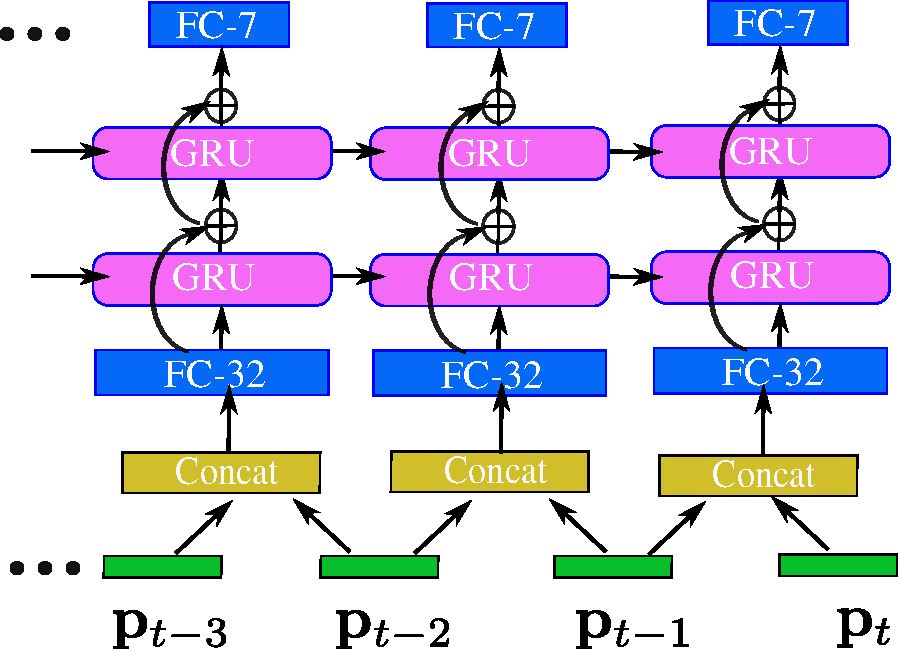
\includegraphics[width=\linewidth]{fig/RNN.pdf}
\end{center}
   \caption{The GRU RNN network architecture for modeling a sequence of camera poses.}
\label{fig:rnn}
\end{figure}

\paragraph{Pose rectify with road prior.} Firstly,

\paragraph{CNN-GRU pose network architecture.}
As shown in \figref{fig:framework}, the CNN of our pose network takes as inputs an image $\ve{I}$ and the rendered label map $\ve{L}^c$ from corresponding coarse camera pose $\ve{p}_i^c$. It outputs a 7 dimension vector $\hat{\ve{p}}_i$ representing the relative pose between the image and rendered label map, and the estimated pose respect the world is $\ve{p}_i = \ve{p}_i^c + \hat{\ve{p}_i}$.
For designing the network, in order to have large kernel to obtain bigger context while keeping the amount of parameters and runtime manageable, we follow the design of Ummenhofer \etal~\cite{ummenhofer2016demon}. The convolutional kernel of this network consists a pair of 1D filters in $y$ and $x$-direction, and the encoder gradually reduces the spatial resolution with stride of 2 while increasing the number of channels. We list the details of the network in our implementation details at \secref{sec:experiments}.

Additionally, after the output pose $\ve{p}_i$ from our pose network, as illustrated in \figref{fig:rnn}, a forward GRU-RNN with residual connection~\cite{wu2016google} is performed to model the temporal motion sequence of the video, since the movement of a vehicle is commonly smooth.
Traditionally in navigation applications of estimating 2D poses,  Kalman filter~\cite{kalman1960new} is applied by calculating either constant velocity or acceleration.
In our case, transition of camera poses is learned from the training sequences, where the current motion is predicted by the RNN from a sequence of previous predicted poses, which yields further improvement over the estimated poses from the pose CNN.


\paragraph{Pose loss.}
Following the PoseNet~\cite{}, we use the geometric matching loss for training, which avoids the balancing factor between rotation and translation.
Formally, given a set of point cloud in 3D $~\hua{P}=\{\ve{x}\}$, and the loss for each image is written as,
\begin{align}
L(\ve{p}, \ve{p}^*) = \sum_{\ve{x} \in \hua{P}}\omega_{l_\ve{x}}|\pi(\ve{x}, \ve{p}) - \pi(\ve{x}, \ve{p}^*)|_2
\label{eq:proj_loss}
\end{align}
where $\ve{p}$ and $\ve{p}^*$ are the estimated pose and ground truth pose respectively. $\pi()$ is a projective function that maps a 3D point $\ve{x}$ to 2D image coordinates. $l_\ve{x}$ is the semantic label of $\ve{x}$ and $\omega_{l_\ve{x}}$ is a weight factor depended on the semantics. Here, we set stronger weights for point cloud belong to certain classes like traffic light, and we found it gives better performance for estimated poses.
In ~\cite{kendall2017geometric}, usually the 3D points that is visible by the camera are used which helps the stableness of learning. In our case, online searching the visible ones in millions of points are infeasible.
Thus, we pre-render a depth map for each training image with resolution of $256 \times 304$, using the ground truth pose, and select those points projected on the depth map for training.

% Intuitively, we find the amount of points in each class is dramatically unbalanced, and most points are those on roads and trees. Nevertheless, the appearance variation of road and trees are not very sensitive to pose changes in the street-view scenario. In order to encourage the network to discover more str
% Thus,  other structures images like electricity pole or road light have rich structures like edges and textures, which potentially should be valued more for matching.
% In~\cite{ummenhofer2016demon}, the model try to predict a flow confidence map revealing the texture rich regions which helps pose estimation. In our work, we adopt the labelled semantic labels, and reweight each 3D point in the training loss, which drives the network to focus more on
% Thus, the learning loss changed to
% \begin{align}
% L(\ve{p}, \ve{p}^*) = \sum_{\ve{x} \in \hua{P}}\omega_{l_\ve{x}}|\pi(\ve{x}, \ve{p}) - \pi(\ve{x}, \ve{p}^*)|_2
% \label{eq:proj_loss}
% \end{align}
% where $\omega_{l_\ve{x}}$ is the weight of class $l_\ve{x}$. We set the weight for each class depends on the class edgeness which is the percentage of pixel along the edge
\subsection{Video parsing with pose guidance}
\label{subsec:parsing}
Having rectified pose at hand, one may direct render the semantic 3D world to current view of a camera, yielding a semantic parsing of the current image. However, the estimated pose is not perfect, thus alignment of very think regions like light pole can totally fail. Another fact is that many LIDAR points are missing due to reflection, \eg regions of building mirrors, and points can be sparse at long distance. Finally, non-linear distortion of images and 3D map could happen due to system error, yielding scene miss alignment. Thus, we propose to a parameter light segment network to handle these issues.
In our experiments, we show with pose rendered label map as an additional input, the segment results are temporally more consistent and yields better accuracy.

\begin{figure*}[]
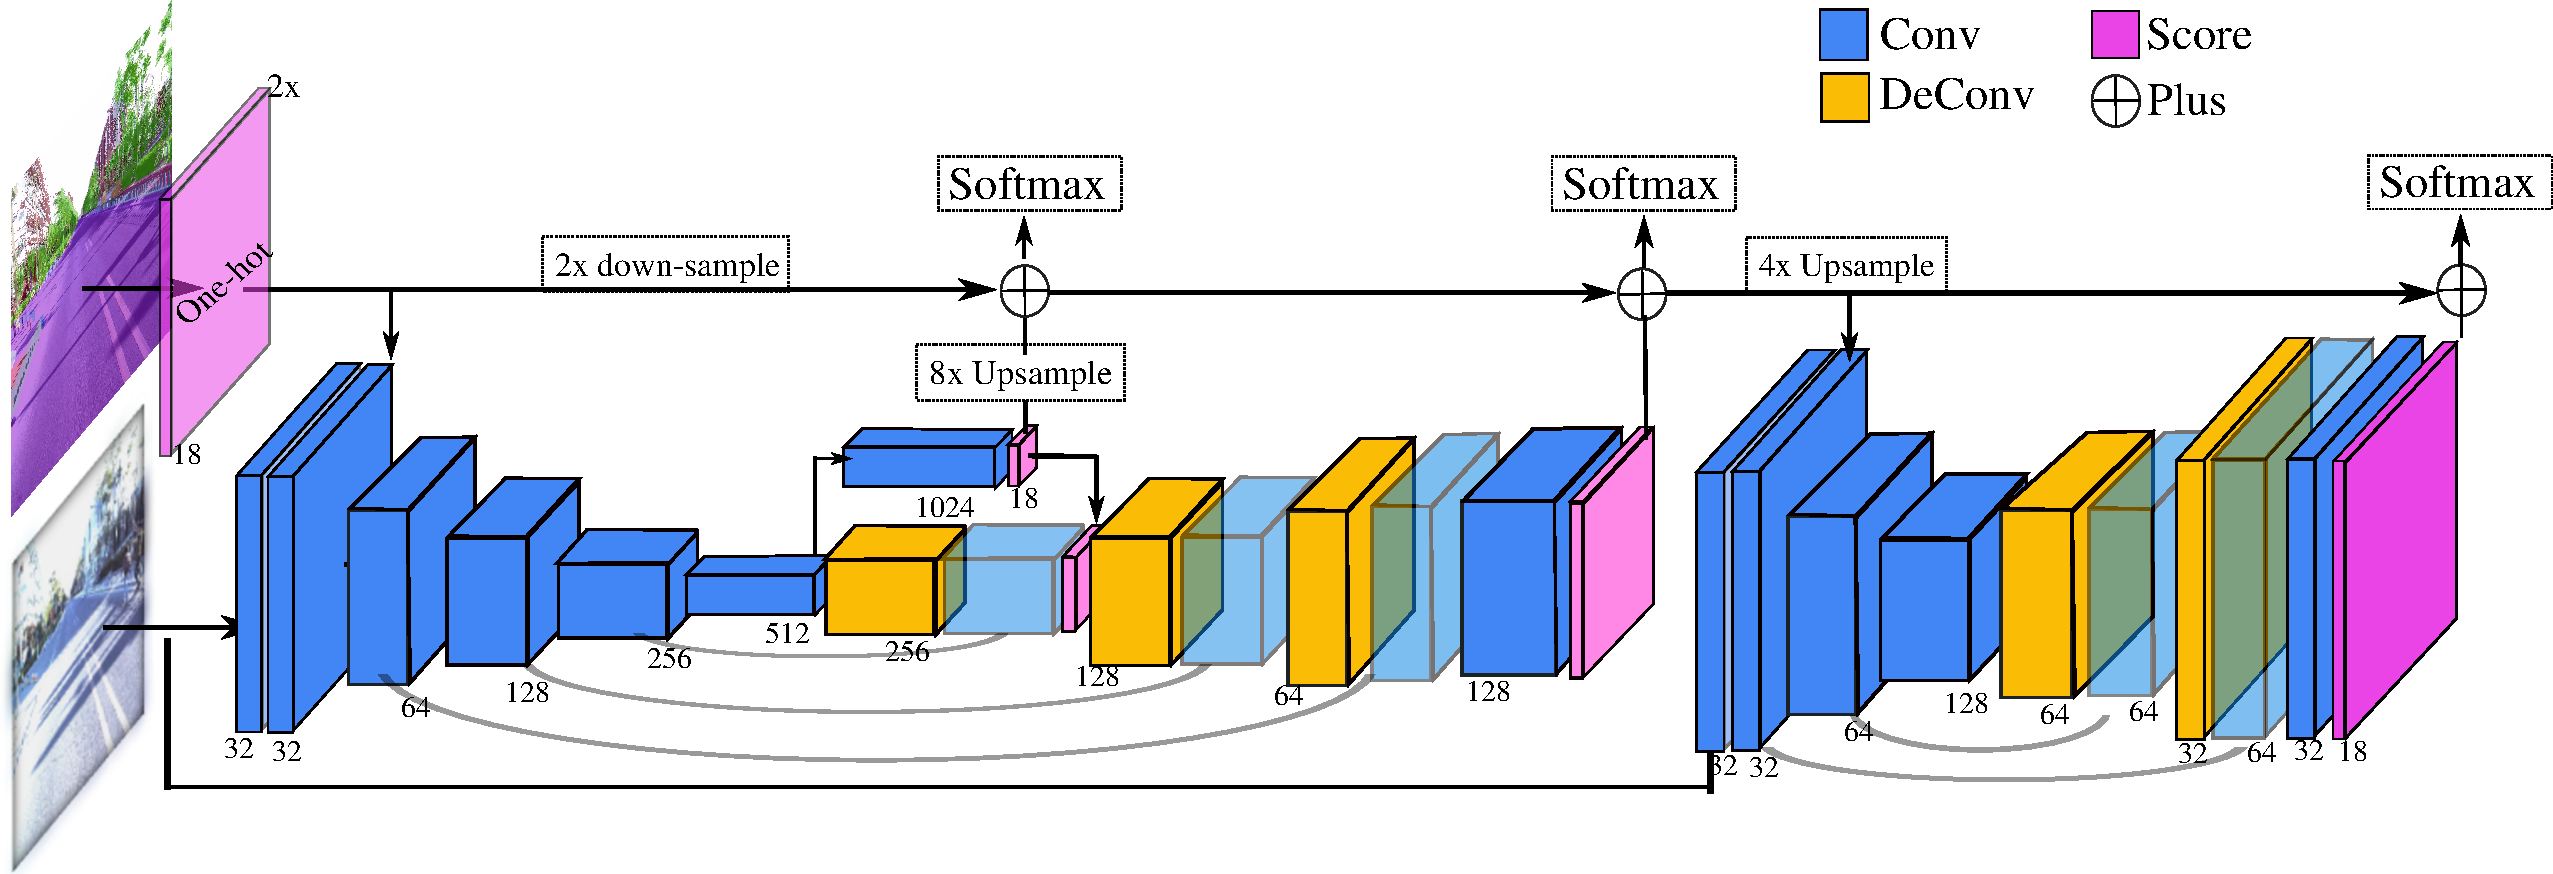
\includegraphics[width=\textwidth]{fig/segCNN.pdf}
\caption{Architecture of the segment CNN with rendered label map as a priori. At bottom of each block, we show the filter size, and at top we mark the rates of downsampling \wrt the input image size. Details are in \secref{subsec:parsing}.}
\label{fig:segnet}
\end{figure*}

\paragraph{Segment network architecture.} As illustrated in \figref{fig:segnet}, the segment network contains an encoder-decoder network and a refinement network, and both have similar architecture with the corresponding ones used in DeMoN~\cite{ummenhofer2016demon}. However, due to we have a segment prior from the 3D map, we add a residual stream (top part of \figref{fig:segnet}), which enourages the network to learn the differences. In~\cite{pohlen2016full}, a full resolution stream is used to keep spatical details, while in our case, the rendered label map provides both semantic and spatial structure informations.
Another notable difference for encoder-decoder network is that for network inputs, rather than directly concatenate the label map with input image, to balance the two, we first transform the label map to a score map through one-hot operation, and embed the score of each pixel to a 32 dimensional feature vector. Then, we concatenate this feature vector with output features from those of the first layer, and keeps the rest as the same with that in~\cite{ummenhofer2016demon}. For refinement network, we use the same strategy to handle the two inputs. Finally, the segment network produce a score map, yielding the semantic label of each pixel.

We train the segment network firstly with only RGB images, then fine-tune the network by adding the input of rendered label maps. This is because our network is trained from scratch, thus needs large amounts of data to learn effective features from the image. However, in our experiments, the rendered label map from the estimated pose has on average 82$\%$ pixel accuracy. This could easily drive the network fitting the input label map at first, while slow down the process towards learning features from images. Finally, for segmentation loss, we use the standard softmax loss, and add intermediate supervision right after the output from encoder and decoder as indicated in \figref{fig:segnet}. 